\documentclass[tikz,border=10pt]{standalone}
\usepackage{tikz}
\begin{document}
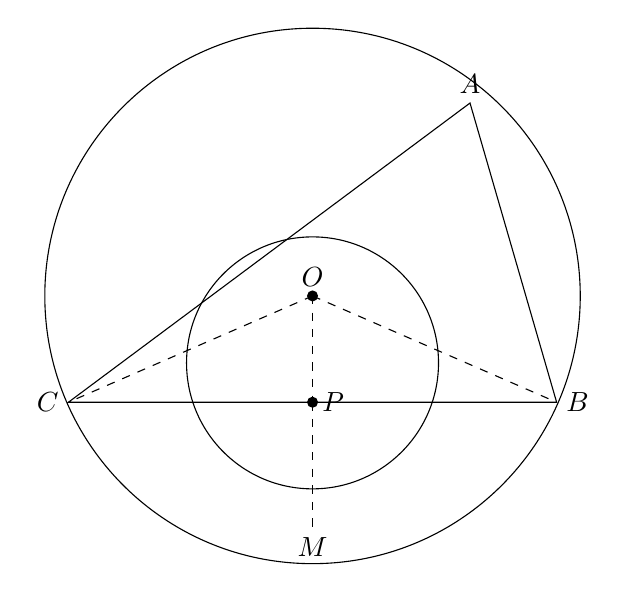
\begin{tikzpicture}[scale=1]

% Coordinates
\coordinate (O) at (0,0.8);
\coordinate (A) at (2.0,3.25);
\coordinate (B) at (3.1,-0.55);
\coordinate (C) at (-3.1,-0.55);
\coordinate (P) at (0,-0.55);
\coordinate (M) at (0,-2.15);

% Auxiliary coordinate for the small circle center (unlabeled in the figure)
\coordinate (S) at (0,-0.05);

% Outer circle
\draw (O) circle [radius=3.4];

% Triangle
\draw (A) -- (B) -- (C) -- cycle;

% Chord through C and B
\draw (C) -- (B);

% Small circle
\draw (S) circle [radius=1.6];

% Dashed segments
\draw[dashed] (O) -- (C);
\draw[dashed] (O) -- (B);
\draw[dashed] (O) -- (P);
\draw[dashed] (P) -- (M);

% Points
\fill (O) circle (2pt);
\fill (P) circle (2pt);

% Labels
\node[above] at (A) {$A$};
\node[right] at (B) {$B$};
\node[left] at (C) {$C$};
\node[above] at (O) {$O$};
\node[right] at (P) {$P$};
\node[below] at (M) {$M$};

\end{tikzpicture}
\end{document}
